\documentclass[tikz]{standalone}
\usepackage{pgfplots}
\usepackage{tikz}
\usepackage{xcolor}
\pgfplotsset{compat = 1.16}
\tikzstyle{format} = [rectangle, draw, fill = blue!20]
\usetikzlibrary{er,positioning}

\begin{document}
    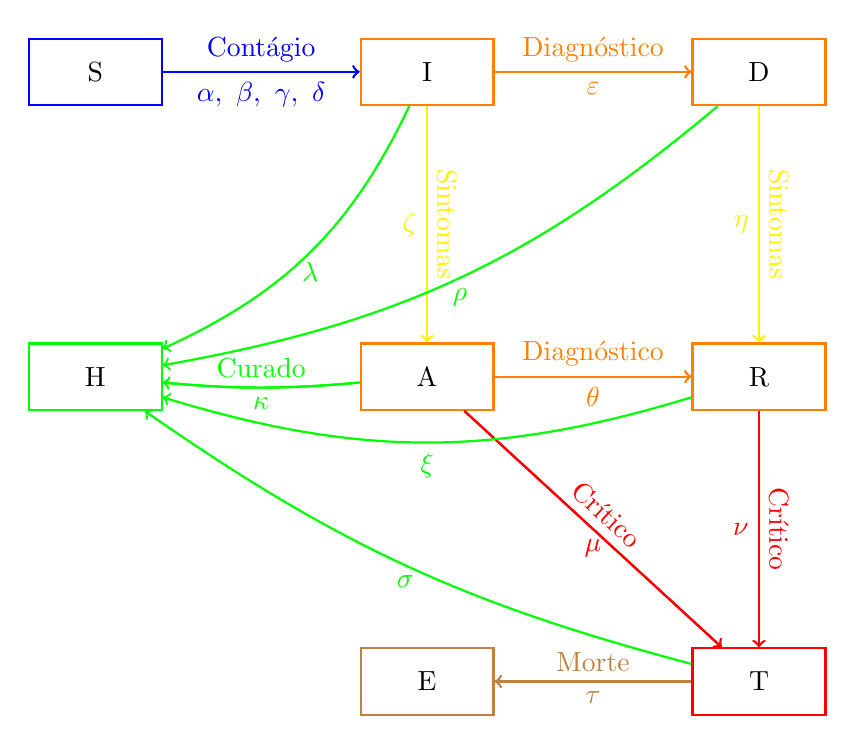
\begin{tikzpicture}[edge from parent/.style = {draw, -latex}]
        \node [entity, draw = blue, thick] (S) {S};
        \node [entity, draw = orange, thick] (I) [right = 2.5cm of S] {I};
        \node [entity, draw = orange, thick] (D) [right = 2.5cm of I] {D};
        \node [entity, draw = orange, thick] (R) [below = 3cm of D] {R};
        \node [entity, draw = orange, thick] (A) [left = 2.5cm of R] {A};
        \node [entity, draw = green, thick] (H) [left = 2.5cm of A] {H};
        \node [entity, draw = red, thick] (T) [below = 3cm of R] {T};
        \node [entity, draw = brown, thick] (E) [left = 2.5cm of T] {E};
        
        \path[->]
            (S) edge [blue, thick] node[below] {$\alpha, ~\beta, ~\gamma, ~\delta$} (I)
                edge [blue, thick] node[above] {Contágio} (I)
            (I) edge [orange, thick] node[below] {$\varepsilon$} (D)
                edge [orange, thick] node[above] {Diagnóstico} (D)
                edge [yellow, thick] node[left] {$\zeta$} (A)
                edge [yellow, thick] node[sloped, above] {Sintomas} (A)
                edge [bend left = 20, green, thick] node[below] {$\lambda$} (H)
            (D) edge [yellow, thick] node[left] {$\eta$} (R)
                edge [yellow, thick] node[sloped, above] {Sintomas} (R)
                edge [bend left = 15, green, thick] node[below] {$\rho$} (H)
            (A) edge [bend left = 5, green, thick] node[sloped, above] {Curado} (H)
                edge [bend left = 5, green, thick] node[below] {$\kappa$} (H)
                edge [orange, thick] node[above] {Diagnóstico} (R)
                edge [orange, thick] node[below] {$\theta$} (R)
                edge [red, thick] node[sloped, above] {Crítico} (T)
                edge [red, thick] node[below] {$\mu$} (T)
            (R) edge [red, thick] node[sloped, above] {Crítico} (T)
                edge [red, thick] node[left] {$\nu$} (T)
                edge [bend left = 17, green, thick] node[below] {$\xi$} (H)
            (T) edge [brown, thick] node[above] {Morte} (E)
                edge [brown, thick] node[below] {$\tau$} (E)
                edge [bend left = 10, green, thick] node[below] {$\sigma$} (H);
    \end{tikzpicture}
\end{document}